\section{Fotos}
Ein von uns gewählter Schwerpunkt bei der Gestaltung der Parallax- Scrolling Website, liegt in der fotografischen Darstellung der Protagonisten und den Umgebungen, in denen sich diese bewegen. Hierbei war es wichtig, dass die Fotos eine hohe Qualität hatten und ästhetisch zueinander passten, damit sich Protagonist und Szenerie gut zusammenführen lassen. Um dies zu ermöglichen, wurde ein Model engagiert, welches jegliche verlangte Pose, in unterschiedlichen Outfits, einnehmen konnte. Diese Umsetzung geschah in Zusammenarbeit mit dem Fachbereich Design. Auf diese Weise konnten mit professionellem Equipment in einer sogenannten Hohlkehle gut beleuchtete, qualitativ hochwertige Fotos für die Website geschossen werden.
Bei den verwendeten Hintergrundbildern handelt es sich um ausgewählte Adobe Stock Fotos, die aufgrund der Quelle ebenfalls eine hohe Qualität aufweisen. 
\begin{figure}[H]
	\centering
	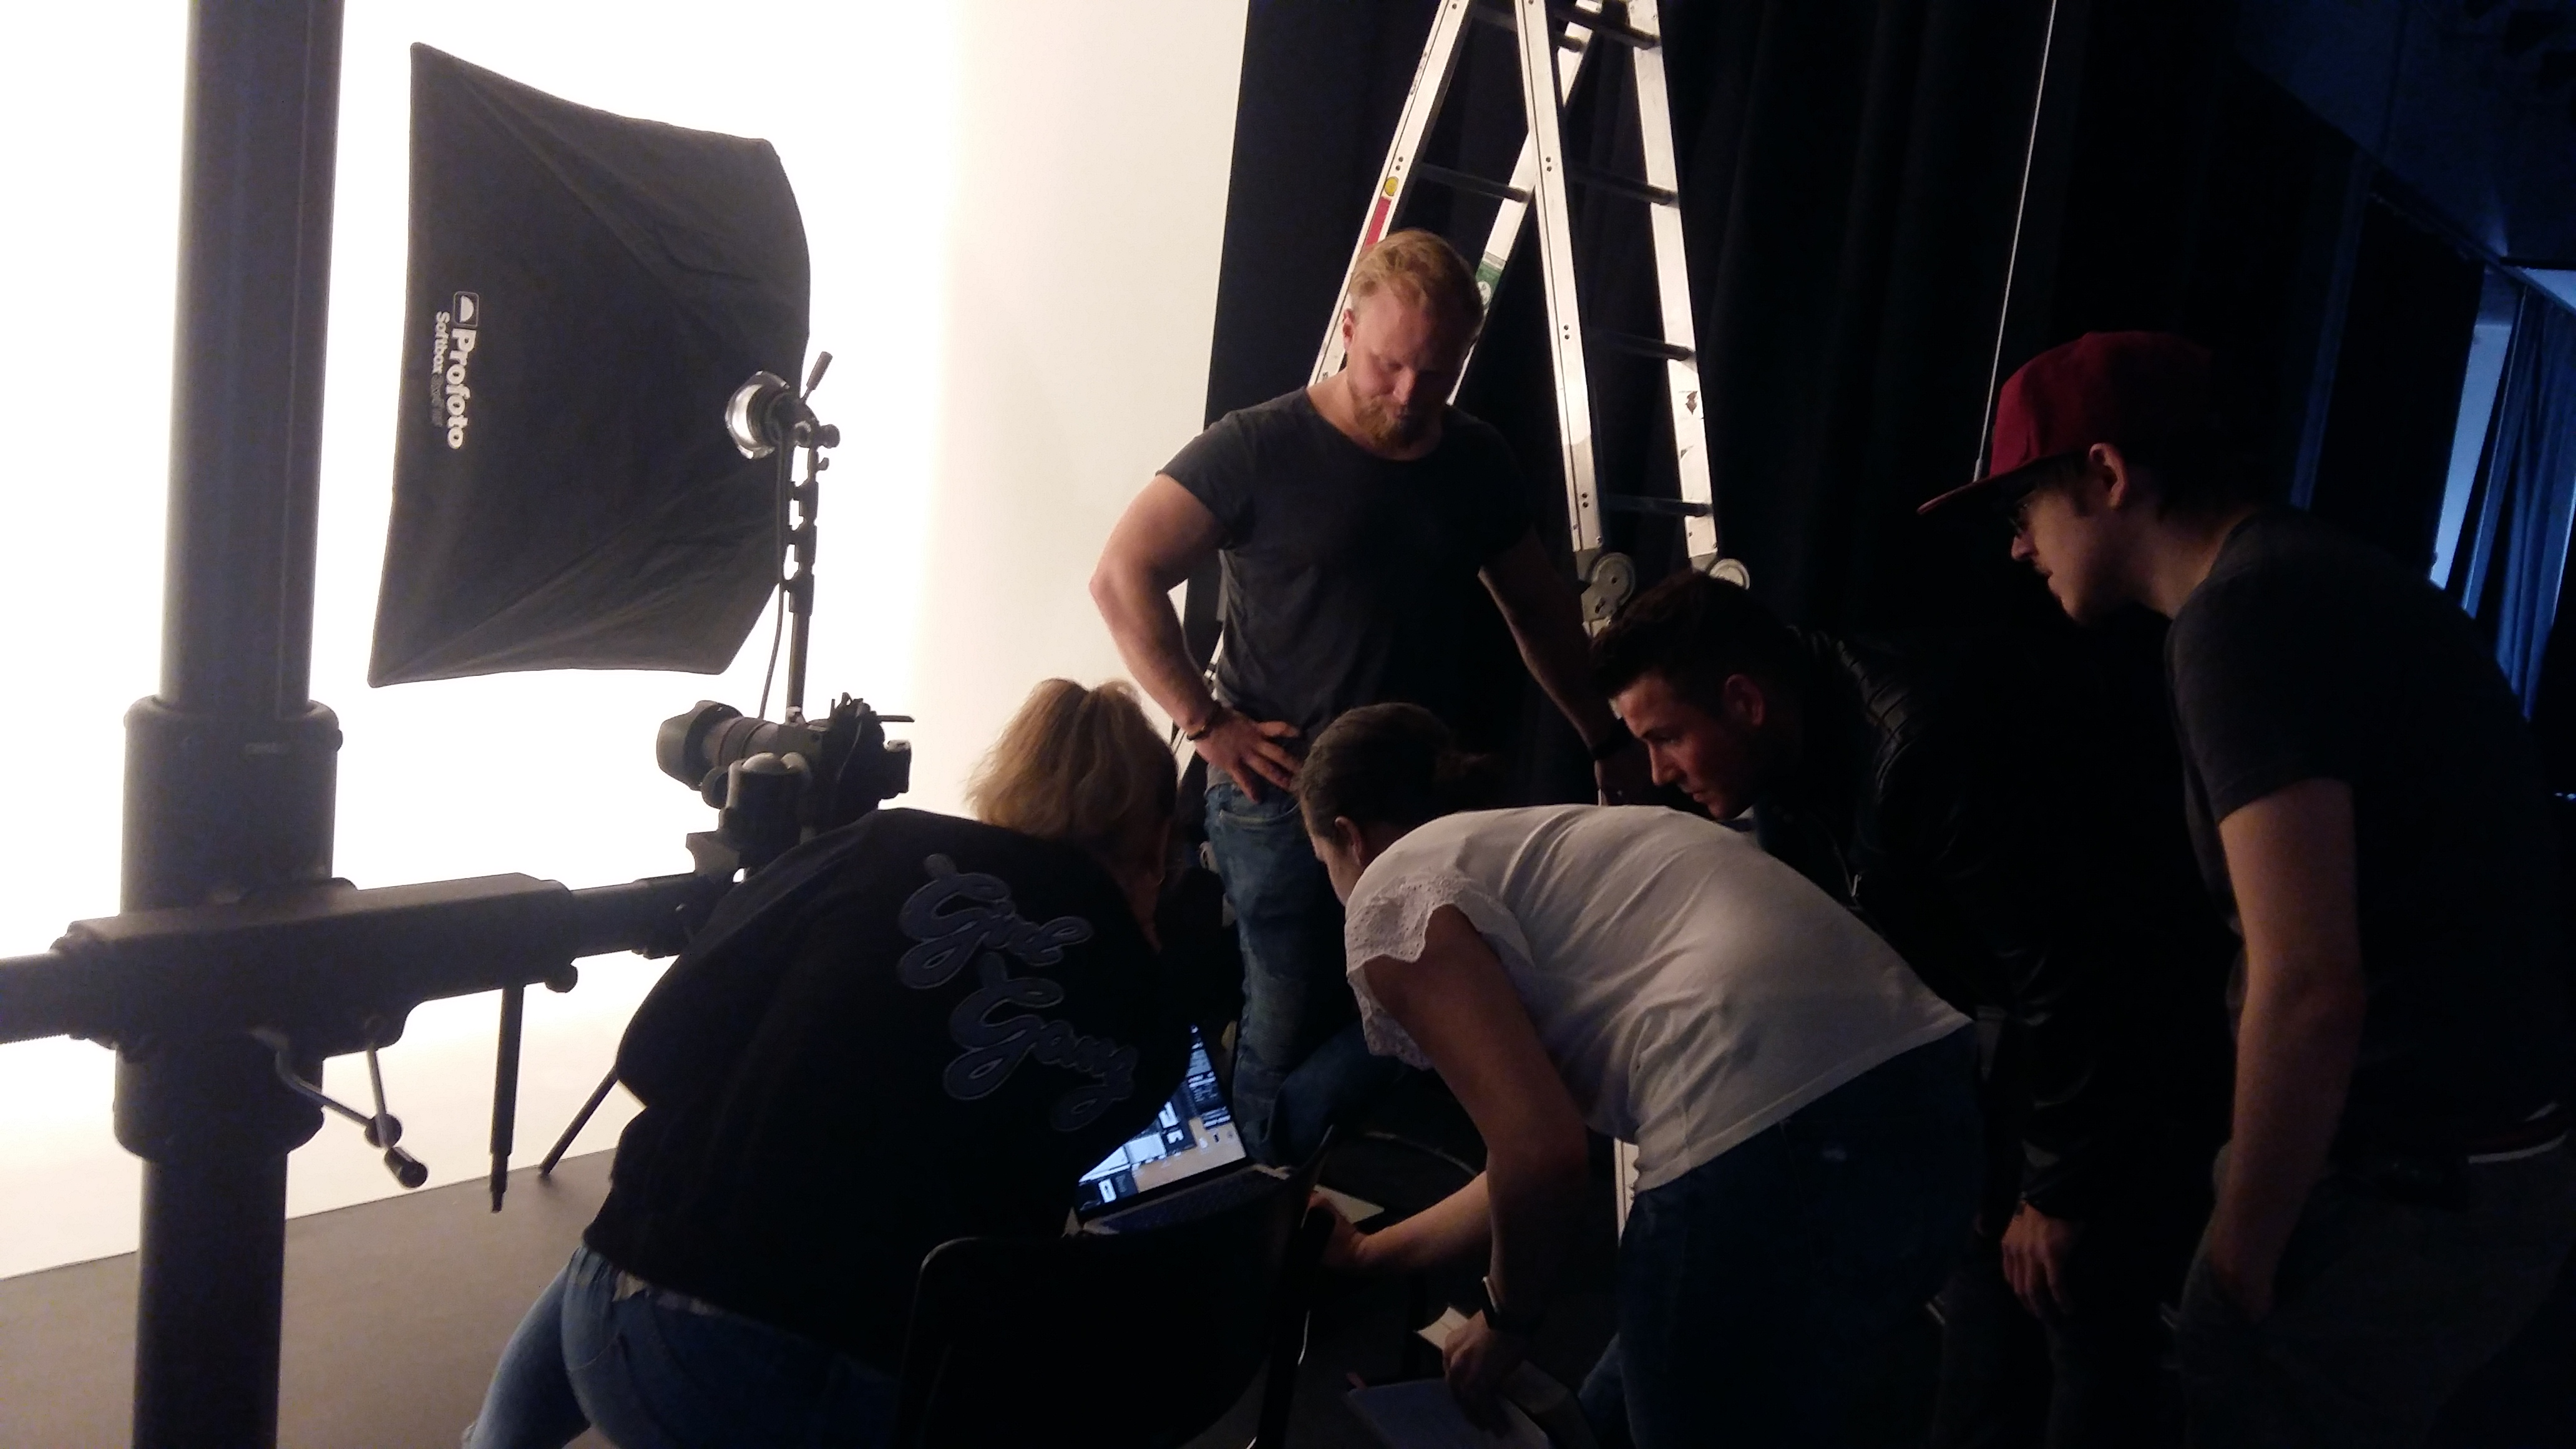
\includegraphics[width=0.7\textwidth]{ProjektFotos}
	\caption{Die Gruppe mit dem Model beim Fotoshooting,\\ Gebäude Design\label{ProjektFotos}}
\end{figure}